\documentclass[11pt]{article}
\usepackage{amsmath, amssymb}
\usepackage{geometry}
\geometry{margin=1in}
\usepackage{fancyhdr}
\usepackage{lastpage}
\usepackage{parskip} % Better paragraph spacing
\usepackage{titlesec} % Better section formatting
\usepackage{graphicx}
\usepackage{float}
\usepackage[most]{tcolorbox}
\usepackage{lmodern}
\usepackage{caption}
\usepackage{listings}

\lstdefinestyle{terminal}{
    backgroundcolor=\color{gray!10}, % light gray background
    basicstyle=\ttfamily\small,
    frame=single, % adds a border
    rulecolor=\color{black},
    breaklines=true
}

% Define commands for reusable content
\newcommand{\coursename}{COM-402 Information Security and Privacy}
\newcommand{\lecturenum}{03}
\newcommand{\lecturedate}{\today}
\newcommand{\professor}{Mathis Payer}

% Configure section spacing
\titlespacing*{\section}{0pt}{2ex plus 1ex minus .2ex}{1.5ex plus .2ex}
% Header / Footer
\pagestyle{fancy}
\fancyhf{}
\fancyhead[L]{\coursename}
\fancyhead[R]{Lecture \lecturenum}
\fancyfoot[L]{EPFL - Computer Science}
\fancyfoot[C]{Author: Jonathan Dutoit}
\fancyfoot[R]{Page \thepage\ of \pageref{LastPage}}

\begin{document}

\begin{center}
  {\large EPFL - Computer Science} \\[0.5em]
  {\Large \textbf{\coursename}} \\[0.5em]
  {\large Lecture \lecturenum\ --- \lecturedate} \\[0.5em]
  {\large Author: Jonathan Dutoit} \\[0.5em]
  {\large Professor: \professor} \\[0.5em]
\end{center}

\vspace{2cm}
\begin{center}
  {\LARGE \textbf{Access Control}}
\end{center}

\vspace{1cm}

\section*{Learning Goals}
\begin{itemize}
	\item Know authentication factors (password, device, biometrics), strengths and risks
	\item Differentiate and identify access control policies (RBAC, DAC, MAC)
	\item Understand the value of authentication protocols and delegated authentication
\end{itemize}

\vspace{1cm}

\begin{center}
  {\LARGE \textbf{Authentication}}
\end{center}

\vspace{1cm}

\section*{What is authentication?}

Authentication is the process of \textbf{verifying} someone's or something's \textbf{identity}

Identification is the act of identifying a particular user (a subject), often named through a username. 

\section*{Password-Based Authentication}

\begin{itemize}
	\item Simplest form of \textit{Authentication}
	\item User sends both username and password to the server, server authenticates user's identity. 
\end{itemize}

\begin{tcolorbox}[
  colback=orange!15,     % background color
  colframe=black!50,    % border color
  boxrule=1pt,       % border thickness
  arc=3mm,             % rounded corners
  left=4mm, right=4mm, top=2mm, bottom=2mm % padding
]
What if the network is compromised? What if the server is compromised?
\end{tcolorbox}

\section*{Authentication Factors}

Access control only makes sense if \textbf{subjects} are authenticated. 

There are 3 common flavours to authenticate subjects

\begin{itemize}
	\item Something you \textbf{know}: password, pin codes
	\item Something you \textbf{own}: paper card, smartphone, certificate, electronic token
	\item Something you \textbf{are}: biometrics
\end{itemize}

Two factor authentication (aka 2FA) requires the use of two factors
\begin{itemize}
	\item A password is often one of the two factors
\end{itemize}

\section*{The Password is Dead...}

"They just don't meet the challenge for anything you really want to secure" (Bill Gates, 2004)

"Within 5 years, you'll never need a password again" (IBM, 2011)

"Passwords are done at Google" (H. Adjins, manager of Information Security at Google, 2013) 

\textbf{Truth}: passwords are still the main form of authentication on the web. 

"No other single technology matches their combination of cost, immediacy and convenience" (C. Herley, P. van Oorschot)

\section*{Even Strong Passwords Are at Risk}

A stolen password can be replayed by anybody

An attacker can: 

\begin{itemize}
	\item Steal passwords using client-side malware
	\item Obtain passwords by cracking hashes stolen from a server
	\item Phish passwords with a fake website
	\item Eavesdrop the password (remember, that's why we need TLS)
\end{itemize}

Attack vector: "Credential stuffing"

\begin{itemize}
	\item Lists of usernames and passwords are distributed online
	\item Hackers try the same credentials on many different sites
	\item Sony and Gawker were both hacked: "Two thirds of people with accounts at both Sony and Gawker reused their passwords"
\end{itemize}

\section*{Password Managers}

Store all your credentials in encrypted form

\begin{itemize}
	\item Your \textbf{master password} is used to decrypt the credentials
	\item To be used on different devices, the encrypted credentials must be accessible online
\end{itemize}

Where are passwords stored?

\begin{itemize}
	\item Password manager works \textbf{offline}, uses a local file (e.g., Keepass)
		\begin{itemize}
			\item You can choose to hist this file in the cloud
		\end{itemize}
	\item Password manager talks to \textbf{a server in the cloud} (e.g., Lastpass)
		\begin{itemize}
			\item Browser plug-in or app downloads credentials and decrypts them locally
			\item You must trust them to not steal your master password
		\end{itemize}
	\item Best of both: the password manager comes with an open source server that you can host where you want (e.g., Bitwarden) 
\end{itemize}

\section*{Authentication/Session Cookies}

After logging in a web application the server sends a cookie, stored in the client

The cookie is kept by the client and used for authenticating against the server

The cookie should be unique for every subject

The cookie can be used by illegal clients through forging

\begin{itemize}
	\item If the server encrypt the cookie it limits forging (HMAC)
\end{itemize}

\section*{Something You Own}

Typically called a (hardware/software) token

Bingo card
\begin{itemize}
	\item Proves that the user owns the card
	\item Can be easily copied without being detected 
\end{itemize}

One time password (OTP) token

\begin{itemize}
	\item Displays a password to be used only once
	\item The password changes with time or click
	\item Proves that user owns token at time of login
	\item Cannot be copied easily (secure hardware)
	\item OATH standard
\end{itemize}

TAN generator
\begin{itemize}
	\item A calculator that generates a number based on user input
	\item Can be used to sign a transaction (Transaction Authentication Number, TAN)
	\item Proves that user owns the generator
	\item Based on a smartcard (secure hardware), typically your bank card
\end{itemize}

Smartphone
\begin{itemize}
	\item OTP is sent by SMS or
	\item OTP is generated by app, as with an OTP token
		\begin{itemize}
			\item Attack: clone the seed and then attack the 2nd factor that way. If the cost is higher than the benefit of security, then users are going to find a way around it (often less safer)
		\end{itemize}
	\item Proof that user owns the phone (or sim card, secure hardware?)
\end{itemize}

\begin{tcolorbox}[
  colback=orange!15,     % background color
  colframe=black!50,    % border color
  boxrule=1pt,       % border thickness
  arc=3mm,             % rounded corners
  left=4mm, right=4mm, top=2mm, bottom=2mm % padding
]
What are the tradeoffs?
\end{tcolorbox}


A private key in a hardware token
\begin{itemize}
	\item Token signs a challenge
	\item Different keys for different websites
	\item Proof that user owns the token
	\item Secure hardware
	\item Universal 2nd Factors (U2F) standard
\end{itemize}

\section*{OATH, Generation of OTP}

\textbf{OATH} (initiative for open authentication)  is a standard that describes:
\begin{itemize}
	\item how OTPs are generated from a seed
	\item an XML format for importing the seeds into an authentication server
\end{itemize}

Standard OATH tokens exist in both hardware or software form
\begin{itemize}
	\item E.g., the Google Authenticator app
\end{itemize}

Generation of the next OTP is either counter or time based (RFC 4226)

\section*{OATH Algorithms}

Counter based: 
\[
hotp(k, c) = truncate(hmac-sha512(k,c))
.\] 

Time-based (initial time $t0$, time interval  $x$):
 \[
totp(k, t) = hotp(k, (t - t0)/x)
.\] 


\begin{tcolorbox}[
  colback=orange!15,     % background color
  colframe=black!50,    % border color
  boxrule=1pt,       % border thickness
  arc=3mm,             % rounded corners
  left=4mm, right=4mm, top=2mm, bottom=2mm % padding
]
What are the tradeoffs between hotp and top? \\

\textbf{Discussion}: \\

\textit{Counter based}: it needs to be synchronized. They could be out of sync due to individual operations that could lead out of sync scenarios \\

\textit{Time-based}: suppose the time is synchronized, replay attacks become a problem if the time interval is big enough. 
\end{tcolorbox}

\section*{RSA SecureIDs}

Secure IDs implement a form of totp

Requires a random seed to be synced between devices and customers

In a massive hack, attackers stole ALL seeds from RSA. The first true supply chain attack

\section*{U2F, FIDO2}

\textbf{Universal 2nd Factor} is a standard developed by the \textbf{FIDO} alliance

Latest version is FIDO2

For each application, the token generates a key pair and gives the public key to the server

\begin{itemize}
	\item On login, the server sends a random challenge to the client
	\item The client signs (the challenge + the domain name of the server + a signature counter)
	\item The client sends the data and signature to the server
	\item The server verifies the signature
\end{itemize}

Adding the domain prevents phising attacks

Adding a counter detects cloning of the private key/replay attack

% Quick centered image
\begin{figure}[H]
    \centering
    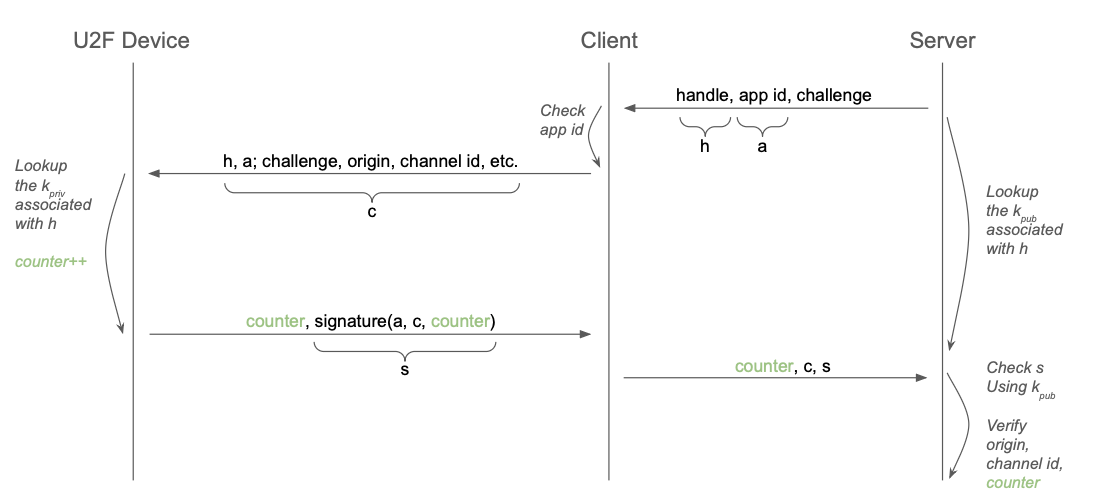
\includegraphics[width=1\textwidth]{u2fworkflow}
    \label{fig:LABEL}
\end{figure}


\section*{U2F, FIDo2 (WebAuthn)}

FIDO2 standardizes U2F within the browser with JavaScript (called WebAuthn) 

Additionally makes use of \textbf{CTAP} to access the signature 

CTAP, the Client to Authenticator Protocol, describes how an application can ask an authenticator to generate an assertion (signature) 

\begin{itemize}
	\item Authenticator can be a 
		\begin{itemize}
			\item USB token
			\item Smartphone connected by Bluetooth
			\item Authentication module of platform (e.g., phone's biometric authentication) 
		\end{itemize}
\end{itemize}

The assertion contains information whether the user

\begin{itemize}
	\item was present (e.g., clicked on a button)
	\item was verified (e.g., pin or fingerprint)
\end{itemize}

\section*{U2F, FIDO2 Pros}

No problem if the server gets hacked:

\begin{itemize}
	\item It is an asymmetric system. The information stored on the server cannot be used to log in
\end{itemize}

No problem if the client gets hacked 

\begin{itemize}
	\item The private key stays in secure hardware of the client
	\item Usage of the key is only possible with user interaction
\end{itemize}

Very convenient 
\begin{itemize}
	\item It can use the native authentication system of the platform (iPhone faceID, Microsfot Hello biometrics, Google fingerprint)
\end{itemize}


\section*{Biometrics}

Motivation
\begin{itemize}
	\item Something you know could be guessed
	\item Something you own could be stolen
	\item Nothing to remember, nothing that can be lost
\end{itemize}

Physiological 
\begin{itemize}
	\item Iris
	\item Retina
	\item Fingerprint
	\item Shape of head
	\item Shape of hand
\end{itemize}

Behavioral
\begin{itemize}
	\item Speech
	\item Keystroke timing
	\item Handwritten signature on tablet
	\item Gait (way of walking)
\end{itemize}


\section*{Biometrics: Authentication Process}

Registration 
\begin{itemize}
	\item Acquisition
	\item Extraction of characteristics
	\item Storage of characteristics
\end{itemize}

Authentication
\begin{itemize}
	\item Acquisition
	\item Comparison
	\item Decision
\end{itemize}

Limitations
\begin{itemize}
	\item Acquisition is never exact
	\item Comparison is never a perfect match
		\begin{itemize}
			\item Biometric information cannot be hashed (due to imprecision in reading out data)
		\end{itemize}
	\item Decision is always error prone
\end{itemize}

\section*{Biometrics: Error Rates}

The decision algorithm must accept a certain error; sensitivity can be tuned

\textbf{FAR} False acceptance rate: the system declares a match when it wasn't 

\textbf{FFR} False rejection rate: the system declares a non-match although it was a match

\textbf{EER} Equal error rate, when the system is tuned such that FAR=FRR

% Quick centered image
\begin{figure}[H]
    \centering
    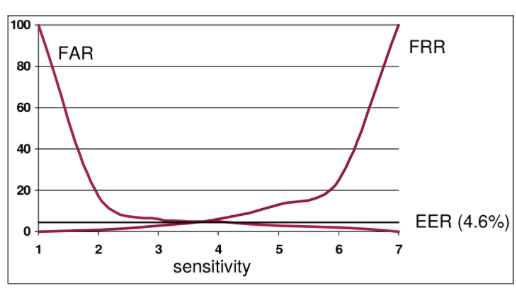
\includegraphics[width=0.5\textwidth]{biometrics-error-rates}
    \label{fig:LABEL}
\end{figure}


\section*{Biometrics: Fingerprints}

The fingerprint is read by a sensor

An image of the ridges is created

The minutiae are extracted at 
\begin{itemize}
	\item termination of a ridge
	\item bifurcation of a ridge
\end{itemize}

A list of coordinates (x, y) and angles is generated

The list is compared with a stored list
\begin{itemize}
	\item the minutiae are shifted and rotated to get the best match
\end{itemize}


\section*{Biometrics: FaceID}
30,000 points are projected on the face and read from a different angle

A specialized and isolated processor constructs a 3D images and compares it to the registered face. Another one is used to store and compare images

\begin{itemize}
	\item The main processor never sees the 3D data
\end{itemize}

The communication with the sensor (camera) is encrypted
\begin{itemize}
	\item cannot be intercepted and replayed
\end{itemize}

This is the same for iPhone fingerprint scanning (Touch ID)
\begin{itemize}
	\item this is why you can't just replace a broken sensor
	\item it has to be paired with the processor
\end{itemize}

Note: you still need to type a password when booting the phone
\begin{itemize}
	\item used to decrypt the storage
\end{itemize}

Limitations: makeup, covid, etc...

\section*{Biometrics Discussion}

Biometrics and authentication
\begin{itemize}
	\item No hashing possible, risk: theft
	\item It is impossible to change a stolen fingerprint!
	\item Best to store the biometric data locally in protected hardware
	\item Example:
		\begin{itemize}
			\item Biometrics are stored in passports, not at the customs offices
			\item Smartphones store fingerprint data in separate, secure hardware
		\end{itemize}
	\item Some sensors can be fooled or replaced
	\item Not ideal for remote authentication
		\begin{itemize}
			\item Rather use it for local access to authentication key (e.g., U2F)
		\end{itemize}
\end{itemize}

Biometrics and privacy
\begin{itemize}
	\item Biometric data is considered sensitive data by European data protection laws and the Swiss law
	\item Biometric data can reveal health issues (e.g., eye pathologies)
	\item Biometrics data can exclude some people (absence of fingerprints or fingers)
	\item A lot of more or less serious research is done with ML and AI to extract information from faces
		\begin{itemize}
			\item Detection of Propensity for Agression based on Facial Structure
			\item Privacy fears as Tokyo taxis use facil recognition cameras to guess riders' age and gender for targeted advertisements
		\end{itemize}
\end{itemize}

\begin{center}
  {\LARGE \textbf{Access control}}
\end{center}

\vspace{1cm}

\section*{Access Control Basics}

After we \textbf{authenticate} a subject...

\textbf{Access control} defines and enforces \textbf{operations} that \textbf{subjects} can do on \textbf{objects}

\begin{itemize}
	\item Bob (subject) has permission to read/write (operation) from a socket (object)
	\item Implies that the subject has been authenticated first
\end{itemize}

\section*{Security Policy}

\textbf{Access rights} (aka permissions, privileges) describe which subjects can do what operations on what objects

A \textbf{security policy} is a collection of access rights. Security policies can be represented as an \textbf{access control matrix}

\section*{Security Mechanism}

\textbf{Security mechanisms} try to prevent operations that are not authorized by the security policy

For example, the kernel implements an access check to see if a user has permissions to open a file. If the access check fails, the rights are not granted. 

Security check is only made when you open the file, the rest of the operations on the file are not checked. 

\section*{Principle of Least Privilege (PoLP)}

\begin{itemize}
	\item Subjects only have the minimum rights required for their job
	\item I.e., subjects are only allowed minimal operations on objects per task
	\item This limits the impact if anything should go wrong
\end{itemize}

The challenge in access control is to have a system that is \underline{simple to implement and manage} and that is \underline{close to the principle of least privilege}

There is no "one size fits all" solution and often different approaches to access control are combined to achieve the best results 

\begin{tcolorbox}[
  colback=green!15,     % background color
  colframe=black!50,    % border color
  boxrule=1pt,       % border thickness
  arc=3mm,             % rounded corners
  left=4mm, right=4mm, top=2mm, bottom=2mm % padding
]
Most important access control principle
\end{tcolorbox}

\section*{Multiple Levels of Access Control}

Network level access control
\begin{itemize}
	\item Subjects are connections or data packets
	\item They are identified by source/destination IP addresses and protocol ports
	\item Typical operations are pass, block, or tag
	\item Example: a database server only accepts traffic from inside EPFL (source addr 128.*.*.*) connecting to TCP port 3306 (mysql)
\end{itemize}

Typically enforced with:
\begin{itemize}
	\item Network equipment: firewalls
	\item The servers:
		\begin{itemize}
			\item Local firewall on the server (e.g., ufw in Linux)
			\item Configuration of the server sofware
		\end{itemize}
\end{itemize}

\begin{tcolorbox}[
  colback=orange!15,     % background color
  colframe=black!50,    % border color
  boxrule=1pt,       % border thickness
  arc=3mm,             % rounded corners
  left=4mm, right=4mm, top=2mm, bottom=2mm % padding
]
What are the tradeoffs of filtering at the different levels
\end{tcolorbox}

Access control at the operating system
\begin{itemize}
	\item Which user can star/stop the DB engine?
	\item Who can read/modify the files of the DB?
\end{itemize}

Access control in the application
\begin{itemize}
	\item Which user of the application can edit user profiles?
	\item Who can see financial data?
\end{itemize}

Access control within the enterprise
\begin{itemize}
	\item Which employees can access the application?
	\item Which application are limited to human resources, which to marketing?
\end{itemize}


\section*{Multiple Approaches to Organize Access Control}

Three common varieties: 
\begin{itemize}
	\item Role-based Access Control (RBAC)
	\item Discretionary Access Control (DAC)
	\item Mandatory Access Control (MAC)
\end{itemize}

\section*{Role-based Access Control (RBAC)}

Simplifies the specification of permissions by grouping users into roles

Centered on user roles (a role can contain multiple permissions)

% Quick centered image
\begin{figure}[H]
    \centering
    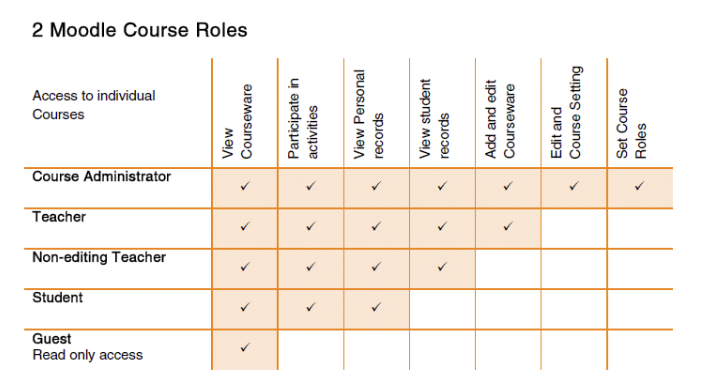
\includegraphics[width=0.7\textwidth]{rbac-example}
    \label{fig:LABEL}
\end{figure}
Example: Operating Systems
\begin{itemize}
	\item Most operating systems have the notion of groups
	\item Groups can be given a set of permissions
	\item Users can be added to groups
	\item Examples:
		\begin{itemize}
			\item Debian/Ubuntu: audio group can access mic and loudspeakers, wireshark group can sniff network traffic
			\item Windows: "remote desktop user" group can access desktop remotely
		\end{itemize}
\end{itemize}

\begin{tcolorbox}[
  colback=gray!15,     % background color
  colframe=black!50,    % border color
  boxrule=1pt,       % border thickness
  arc=3mm,             % rounded corners
  left=4mm, right=4mm, top=2mm, bottom=2mm % padding
]
\textbf{Which groups does your user belong to?}

\vspace{0.3cm}

\verb|id <username>|
\end{tcolorbox}


\begin{minipage}{0.4\textwidth}

\textbf{Pros}:
\begin{itemize}
	\item Easy to grasp the idea of roles
	\item Easy to manage
		\begin{itemize}
			\item Roles decouple digital entities from permissions
			\item Simply assign roles to a new subject. No need to decide for each object
			\item Easy to revoke authorizations by removing role
		\end{itemize}
	\item Easy to tell through roles which permissions a subject has and why. 
		\begin{itemize}
			\item Typically centrally managed
		\end{itemize}
\end{itemize}

\end{minipage}
\begin{minipage}{0.6\textwidth}
\textbf{Cons}

\begin{itemize}
	\item Difficult to decide on the granularity of roles
		\begin{itemize}
			\item Do we need different roles modifying and deleting client information?
			\item Leads either to role explosion or roles that are too broad (not least privilege)
		\end{itemize}
	\item Role meaning is fuzzy
		\begin{itemize}
			\item Employee position in company may be different from RBAC role (think developers in same team working on different subjects)
		\end{itemize}
	\item Unclear if roles can be shared across different departments
		\begin{itemize}
			\item For "manager" roles, in general, is a finance IT manager the same as marketing IT manager?
		\end{itemize}
\end{itemize}
\end{minipage}

\newpage

\section*{Discretionary Access Control (DAC)}

Access control is at the discretion of the object owner
\begin{itemize}
	\item Owner specifies policies to access resources it owns
\end{itemize}

Access control matrix represents rules
\begin{itemize}
	\item stored by \textcolor{blue}{column}: \underline{Access Control List (ACL)} stored with object
	\item stored by \textcolor{purple}{row}: \underline{Capabilities} stored with subjects
\end{itemize}

\section*{DAC in Unix file system}

Stored \textbf{in the target objects}, e,g,m in the metadata of files in the file system

Subjects are grouped in three categories: owner, group, other.

Three access rights: (r)ead, (w)rite, e(x)ecute. The three rights and three groups are stored in 9 bits
\begin{itemize}
	\item represented as three octal digits
	\item owner rwx, group rx, others r: \verb|rwx|r-x|r--| = 754
	\item the permissions of the first matching category dominate
\end{itemize}

\section*{ACLs in Unix: setuid/setgid}

If a program has setuid bit set, it will be run with the permissions of the owner of the file instead of the permissions of the user running the program

Very useful to give users more privileges in specific cases

Example: the passwd command allows a user to modify the \verb|/etc/passwd| and \verb|/etc/shadow| files

\begin{lstlisting}[style=terminal]
ls -l /etc/{passwd,shadow}
-rw-r--r-- 1 root root 2786 avr 23 11:09 /etc/passwd
-rw-r----- 1 root shadow 1489 avr 23 11:09 /etc/shadow
\end{lstlisting}

and the program \verb|/usr/bin/passwd| has the setuid bit
\begin{lstlisting}[style=terminal]
$ ls -l /usr/bin/passwd
-rwsr-xr-x 1 root root 59640 jan 25 2018 /usr/bin/passwd
\end{lstlisting}

Hence when a user Jane runs the program passwd, the process is run as root. 

The setgid bit does the same for groups: the group of the process running the program is set to the group of the owner of the program. 

setuid and setgid are displayed as s instead of x in the access rights of the file.

setuid is very practical, because it lets unprivileged users execute some well defined privileged actions, but it can also be dangerous, why?

$\Rightarrow$ Any bug in programs where the setuid bit is set could be used to escalate the privileges of the user. As the user controls inputs to the program running as root, they may use that input to trigger the bug and gain arbitrary code execution.

\section*{Capabilities in Linux}

Capabilities are permissions that are related to a subject, not to an object

Linux supports capabilities for processes. Some example are: 
\begin{itemize}
	\item \verb|CAP_CHOWN|: make arbitrary changes to file user ID and group ID
	\item \verb|CAP_SYS_BOOT|: user reboot or kexec (load a new kernel)
\end{itemize}


Example: dumpcap is the program used by wireshark to sniff network traffic
\begin{itemize}
	\item it can only be run by user root and member of the wireshark group
	\item It does not have the setuid bit
\end{itemize}

\begin{lstlisting}[style=terminal]
$ ls -l /usr/bin/dumpcap
-rwxr-xr-- 1 root wireshark 104688 jan 19 06:23 /usr/bin/dumpcap

\end{lstlisting}
Let's check the capabilities of dumpcap: 

\begin{lstlisting}[style=terminal]
$ sudo getcap /usr/bin/dumpcap
/usr/bin/dumpcap = cap_net_admin,cap_net_raw+eip
\end{lstlisting}

The process assumes \verb|net_admin| and \verb|net_raw| capabilities when launching \verb|dumpcap|: it can read and write to all network interfaces

The program can do this while running in the name of the user:

\begin{lstlisting}[style=terminal]
$ ps -ef | grep dumpcap
user 24342 26651 0 13:10 pts/1 00:00:00 /usr/bin/dumpcap
\end{lstlisting}
This is much safer than using setuid

If there was a bug in dumpcap allowing to execute arbitrary commands, setuid would run these commands as root!


\section*{DAC Pros and Cons}

\begin{minipage}{0.5\textwidth}
\textbf{Pros}
\begin{itemize}
	\item Flexible
	\item Intuitive
	\item Easy to manage (owners get to set the permissions themselves)
\end{itemize}
\end{minipage}
\begin{minipage}{0.5\textwidth}
\textbf{Cons}
\begin{itemize}
	\item Depends on the owners judgement
	\item Only works if programs are benign and users make no mistakes
	\item Vulnerable to the "Trojan" / declassification problem
\end{itemize}
\end{minipage}

\section*{Mandatory Access Control}

Tries to ensure that even someone with access cannot leak the data

Historically associated with military-grade information security

\begin{itemize}
	\item Multilevel security: e.g., unclassified, confidential, secret, top-secret
\end{itemize}

The system labels both subjects and objects with security labels
\begin{itemize}
	\item Can only be modified by trusted administrators via trusted software
\end{itemize}

Security policy:
\begin{itemize}
	\item Example: Subjects can only access objects of the same or lower level
\end{itemize}

Depends on trusted software and admins for
\begin{itemize}
	\item Keeping the system in a protected state, by preventing operations that violate the rules of the matrix
	\item Labeling new subjects and objects
	\item Perform transitions of labels (e.g., when a document is declassified) 
\end{itemize}

CAN be used in conjunction with DAC or RBAC

\begin{tcolorbox}[
  colback=gray!15,     % background color
  colframe=black!50,    % border color
  boxrule=1pt,       % border thickness
  arc=3mm,             % rounded corners
  left=4mm, right=4mm, top=2mm, bottom=2mm % padding
]
\textbf{Quiz! Why is it a bad idea to allow secret subjects to write confidential documents?}

\vspace{0.3cm}

Remember the order of "secrecy": unclassified, confidential, secret, top-secret \\

A secret subject may read a secret file and write the content into a confidential file, thereby reclassifying the secrecy level and downgrading it. This is also called the "no-write-down" problem.
\end{tcolorbox}

\section*{MAC Confidentiality vs Integrity}

MAC and Confidentiality
\begin{itemize}
	\item When protecting confidentiality, we don't want users to write to a lower level (\textbf{no write-down)}
		\begin{itemize}
			\item Prevents leaking information from higher to lower levels ("trojan")
		\end{itemize}
	\item Typical scenario: network access control
		\begin{itemize}
			\item Network split in zones: internet, internal, secret
			\item Firewalls only allow data to flow from lower zones to higher zones
		\end{itemize}
\end{itemize}

MAC and Integrity

\begin{itemize}
	\item We don't want users from lower levels to write into higher levels (\textbf{no write-up})
		\begin{itemize}
			\item Prevents unauthorized modification of objects
		\end{itemize}
	\item Typical scenarios: operating systems
		\begin{itemize}
			\item Users can read and execute OS programs, but they cannot modify them
		\end{itemize}
\end{itemize}


\begin{minipage}{0.5\textwidth}
\textbf{Pros}
\begin{itemize}
	\item Addresses the limitations of DAC
	\item Easy to scale
\end{itemize}

\end{minipage}
\begin{minipage}{0.5\textwidth}
\textbf{Cons}
\begin{itemize}
	\item Can be too restrictive, prevent legitimate tasks
	\item Not flexible
\end{itemize}

\end{minipage}

\newpage
\begin{center}
  {\LARGE \textbf{Authentication protocols}}
\end{center}

\textbf{When sending a password over TLS is not enough}
\vspace{1cm}

\textbf{Motivation}

Why is the naive Password-based Authentication insufficient?
\begin{itemize}
	\item Sending passwords over network is risky, leaks to adversary when the network is compromised
	\item Attacker may break encryption
	\item Server may be compromised or even store passwords twoo
	\item Challenge-response Authentication
\end{itemize}

Why do we need authentication protocols?
\begin{itemize}
	\item Standardization and save duplicated efforts implementing authentication
	\item Kerberos
\end{itemize}

\section*{Challenge-Response}
Rather than sending the password to the server
\begin{itemize}
	\item The server sends a random challenge to the client
	\item The client uses the password hash to create a response
		\begin{itemize}
			\item E.g., encryption or HMAC of the challenge
		\end{itemize}
\end{itemize}

Typically, challenge response protocols are vulnerable to MITM attacks
% Quick centered image
\begin{figure}[H]
    \centering
    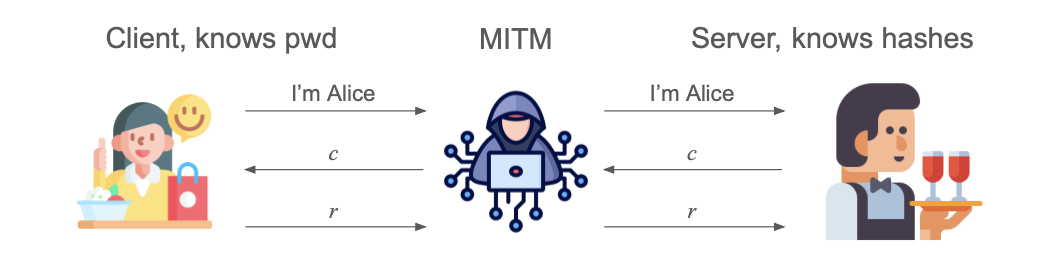
\includegraphics[width=0.8\textwidth]{challenge-response}
    \label{fig:LABEL}
\end{figure}

Microsoft introduced the signature of the packets with a key derived from the pwd hash (it is actually an HMAC)
\begin{itemize}
	\item The MITM does not know the key, cannot send any packets
\end{itemize}

\textbf{Mutual Authentication}

The server and client can both use a challenge: they can authenticate each other. 

Examples:
\begin{itemize}
	\item Newer versions of Microsoft challenge-response (SMBv2)
	\item WiFi WPA, WPA2, and WPA3
\end{itemize}

Challenge-response protocols may be eavesdropped or suffer cracking attacks
\begin{itemize}
	\item The attacker records a challenge and a response
	\item They try all possible password to find which would yield the same response
\end{itemize}

\section*{Kerberos}

Kerberos provides authentication and authorization across a network

Subjects receive tickets that they use to access objects

Exclusively based on symmetric keys

Developed at MIT in the 80's, initially deployed in Unix, the main authentication protocol in Windows LAN networks.

Key idea: delegation
\begin{itemize}
	\item Users authenticate once and then access \textbf{multiple services} without needing to repeatedly re-enter credentials
\end{itemize}

Separation of concerns
\begin{itemize}
	\item Authentication
	\item Access control (Authorization)
	\item Providing actual service
\end{itemize}

% Quick centered image
\begin{figure}[H]
    \centering
    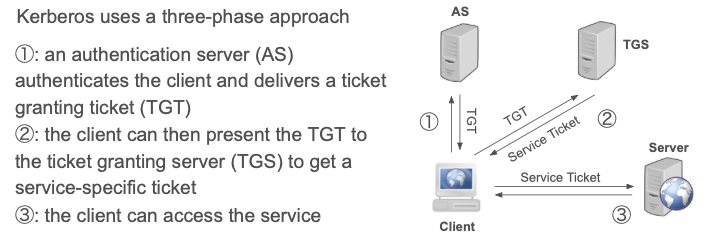
\includegraphics[width=0.8\textwidth]{kerberos}
    \label{fig:LABEL}
\end{figure}

The \textbf{AS} handles \textbf{authentication} (user identity verification and issuing the TGT).
\begin{itemize}
	\item This step is solely about \textbf{confirming} the user's \textbf{identity}.
\end{itemize}

The \textbf{TGS} handles \textbf{access control} (authorization, issuing service-specific tickets based on the TGT)

\begin{itemize}
	\item Once the TGT is issued by the AS, the user doesn't need to go back to the AS for each service access. Instead, the TGT can be used multiple times to request service-specific tickets from the TGS.
\end{itemize}

\newpage

\begin{center}
  {\LARGE \textbf{Delegated authentication}}
\end{center}

\vspace{1cm}

\section*{OAUTH2}

Kerberos is great but targets the intranet. Following the idea of delegated auth... 

Oauth2 (RFC 6749) is used for delegated authentication on the \textbf{Internet}

\begin{itemize}
	\item Oauth2 providers like Facebook, Google, or X/Twitter can be used to authenticate and access other applications
\end{itemize}

\begin{tcolorbox}[
  colback=orange!15,     % background color
  colframe=black!50,    % border color
  boxrule=1pt,       % border thickness
  arc=3mm,             % rounded corners
  left=4mm, right=4mm, top=2mm, bottom=2mm % padding
]
Remeber TLSv1.2 vs 1.3? OAUTH2 is much simpler than Kerberos
\end{tcolorbox}

\section*{Roles}

\textbf{Client}: application that wants to use authentication and possibly access the user's data

\textbf{Resource server}: server that has user's data that client wants to use

\textbf{Authorization server}: server on which the user authenticates

\textbf{User}: Owner of the account and resources on resource server

% Quick centered image
\begin{figure}[H]
    \centering
    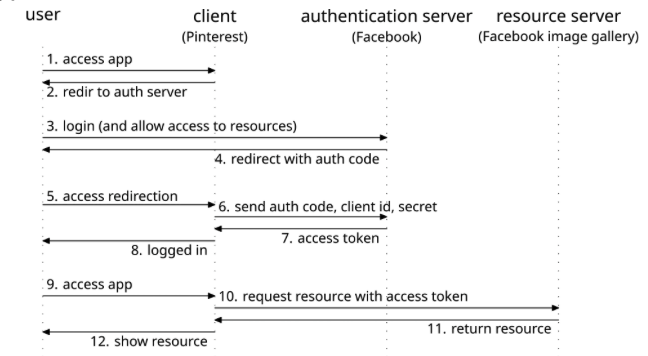
\includegraphics[width=0.8\textwidth]{oauth2}
    \label{fig:LABEL}
\end{figure}

The client and the authentication server have a shared secret
\begin{itemize}
	\item the client thus has to register with the authentication server before being able to offer this service
	\item the secret is used when the client exchanges the \textbf{authentication code} for an \textbf{access token}
	\item the authentication code is not sufficient to get access to the resources
	\item it can only be used by the client and nobody else
\end{itemize}

Oauth2 can be used by browsers or in app
\begin{itemize}
	\item in an app a redirection for authentication can be either
		\begin{itemize}
			\item opening a browser within the app (called a webview)
				\begin{itemize}
					\item not very safe as the app could be spying while you login
				\end{itemize}
			\item switching to the other app (e.g. Facebook) and then back
		\end{itemize}
\end{itemize}

Most apps in smartphones (e.g., X, Instagram, Gmail) do not store your password
\begin{itemize}
	\item The use OAuth2 to request an access token and use it
	\item When you change your password you don't need to type your new password into all your devices
\end{itemize}

\end{document}
